\chapter{Convolutional Neural Network}
Convolutional Neural Networks (CNNs) or Convolutional Networks are similar with the original of Neural Networks. It means that CNNs has also the score function and the loss function at the end of network. However, CNNs are the specialized neural network for preprocessing data that has grid topology \textit{i.e.} time series data can be seen as $1-D$ grid or images data can be presented as $2-D$ grid, \ldots. The networks have the name ``convolutional neural network" means that the networks have implemented \textbf{convolution} operation which is a kined of linear operation. Like neural networks, CNNs receive also the input, then pass them through a series of hidden layers and give the outputs at the last layer. The layers of the CNNs have neurons arranged in 3 dimensions: \textbf{width, height, depth}. In CNNs, some layers contain the parameters but other don't. This chapter will describe the element layers which can be used to build a CNN and how CNNs work.

\section{CNN components}

A CNN is made from the layers. The common layers in CNN are convolutional, nonlinear, pooling and full connected layers. CNN takes image as an input, pass it through the series of layers and get an ouput. Each layer has a different function to transform the input to another layer. 
\begin{figure}[h]
	\centering
	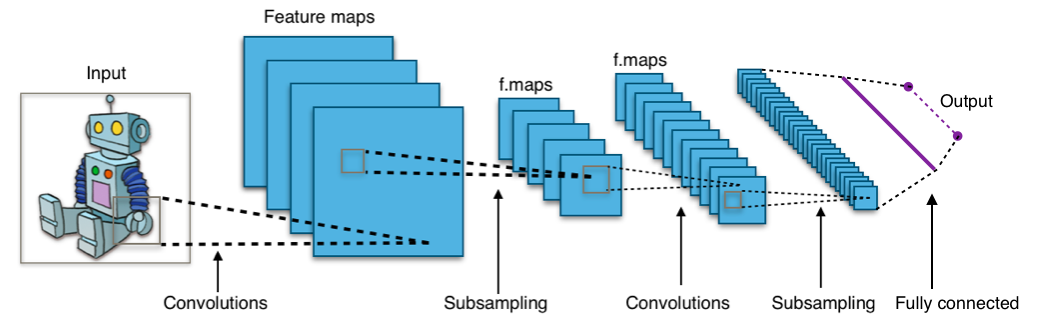
\includegraphics[scale=0.45]{images/cnn_architecture}
	\caption{An architecture of convolutional neural network}
	\label{figlncex}
\end{figure}

\subsection{Convolutional layer}
Convolutional (CONV) layer are one of the main layers in CNNs which is implemented the convolution operation. The convolution operation refers an \textbf{input} and a \textbf{kernel} as the arguments and outputs the \textbf{feature map}. It compute a dot product between the input and the kernel. In practice, the input of the CONV layer oftens the images. The convolution operation is computed for each small region in the input with the kernel. At the output of neurons is combining the result of the connected to local regions.

CONV layer uses a set of learnable filters as parameters. Each filter is small spatially but extends the depth of the input. During the forward pass, the filter is slided over each pixel of the input (from left to right, top to bottom) and calculate dot product between the entries of the filter and the input at this position. During the process, we can see the response of input for each filter such as the orientation of the edge or a blotch of some color on the firt layer. With an entire set of filters in each CONV layer, we will stack these activation maps along the depth dimension and procedure the output volume.

Instead of connecting a neurons to all neurons in the previous layer, CONV connect each neurons to only a local region of the input. The spatial extent of this connectivity is a hyperparameter called the receptive field of the neuron (equal with the number of the filter). The extent of connectivity has the depth axis is equal to the depth of the input. For example, if the input has size [32x32x3] and the filter size is [5x5] then each neuron in the CONV layer will have the weights to a [5x5x3] region in the input, and total of $5*5*3 = 75$ weights. This is the way that each neuron in CONV layer connected to the input; but how many neurons that we have in the output and how the order between the neurons. With 3 hyperparameters \textbf{depth, stride} and \textbf{zero-padding} will help us control the size of the CONV output.
\begin{itemize}
	\item \textbf{Depth}: corresponds to the number of filters we would like to use, each learning to look for something different in the input.
	\item \textbf{Stride}:  which we slide the filter. When the stride is 	1 then we move the filters one pixel at a time. If the stride is 2 (or more), then the filter will jump 2 (or more) at a time when we slide the filter.
	\item \textbf{Zero-padding}: pad the input with zeros arund the border.
\end{itemize}
We can compute the spatial size of the output through the equation:
\begin{equation}
	N = \frac{(W - F + 2P)}{S} + 1
	\label{convneuron}
\end{equation}
Where:
\begin{itemize}
	\item \textbf{W} is the input size
	\item \textbf{F} is the filter size of CONV layer neurons
	\item \textbf{P} is amount of zero padding on the border
	\item \textbf{S} is the stride.
\end{itemize}

The important of equation \ref{convneuron} is the constraint on stride. If we choose the stride inadequate, the result could be not an integer, it means that the neurons do not fit neatly and symmetrically across the input. Besides, using zero-padding also affects to the spatial size of the output. Therefore, the setting of the hyperparameters is considered to cheap, we can throw an exception or use zero pad the rest or crop the input to make it fit,etc. 
Easy to see that if a CONV layer received the input of size $[w x h x d]$, then the number of neurons is $(w * h * d)$; and if the size of the filter on each neuron is $k$, then we have $k * k * d$ weights for each neuron. And the total parameters that we need to keep on the layer is $(w * h * d) * (k * k * d)$, this number is clearly high. To reduce the number of the parameter on the layer, we can assume that if the filter is useful to compute at a position $(x_1,y_1)$, then it should be useful to compute at different postion $(x_2,y_2)$. With this way, we just need to keep unique set of weights for each depth slice(single 2-dimensional slice of depth). This technique is called parameter sharing.\\[0.2cm]
In general, the CONV layer:
\begin{itemize}
	\item Accept a input of size \textbf{$W_1$ x $H_1$ x $D_1$}
	\item Requires four hyperparameters:
		\begin{itemize}
			\item Number of filters \textbf{K}
			\item Size of filter (spatial extent) \textbf{F} (commonly F = 3)
			\item The stride \textbf{S} (commonly S = 1)
			\item The number of zero padding \textbf{P} (commonly P = 1)
		\end{itemize}
	\item The output with size of \textbf{$W_2$ x $H_2$ x $D_s$} where:
		\begin{itemize}
			\item \textbf{$W_2$ = $(W_1 - F + 2P)/S$ + $1$}
			\item \textbf{$H_2$ = $(H_1 - F + 2P)/S$ + $1$}
			\item \textbf{$D_2$ = $K$}
		\end{itemize}
	\item With parameter sharing, CONV layer store \textbf{$F * F * D_1$} weight per filter, for a total of \textbf{$(F * F * D_1) * K$} weights and \textbf{$K$} biases.
	\item In the output, the \textbf{d}-th depth slice (size \textbf{$W_2 x H_2$} is the result of performing a valid convolution on the \textbf{d}-th filter over the input volume with a stride of \textbf{$S$} and then offset by \textbf{d}-th bias.
\end{itemize}
Fig. \ref{figconv} shows an example of convolution layer. It receives an input with the size of $(7 \times 7 \times 1)$. The parameters of layer are set: \textbf{K = 1, F = 3, S = 1, P = 0}. It means the layer used a kernel with the size of $(3 \times 3)$, the stride of each pixel $1$ and zero padding $P = 0$. Therefore, the size of the output volume is $(7 - 3 + 2.0)/1 + 1 = 5$ $([5 \times 5 \times 1])$. The highlight parts present for convolution operation at a region on input: Each element in the output (red) is computed by elementwise multiplying the hightlight of input (yellow) with the kernel (green), summing it up, and then offsetting the sum result by the bias (the bias is zero in this case).

\begin{figure}[!h]
	\centering
	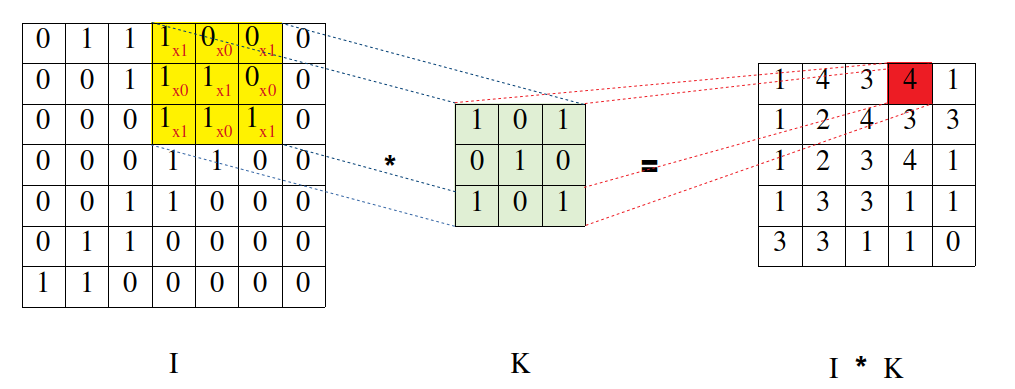
\includegraphics[scale=0.35]{images/convolutional}
	\caption{Convolution operation of a $(7 \times 7)$ matrix and kernel of $(3 \times 3)$}
	\label{figconv}
\end{figure}
\iffalse
\begin{figure}[!h]
	\centering
	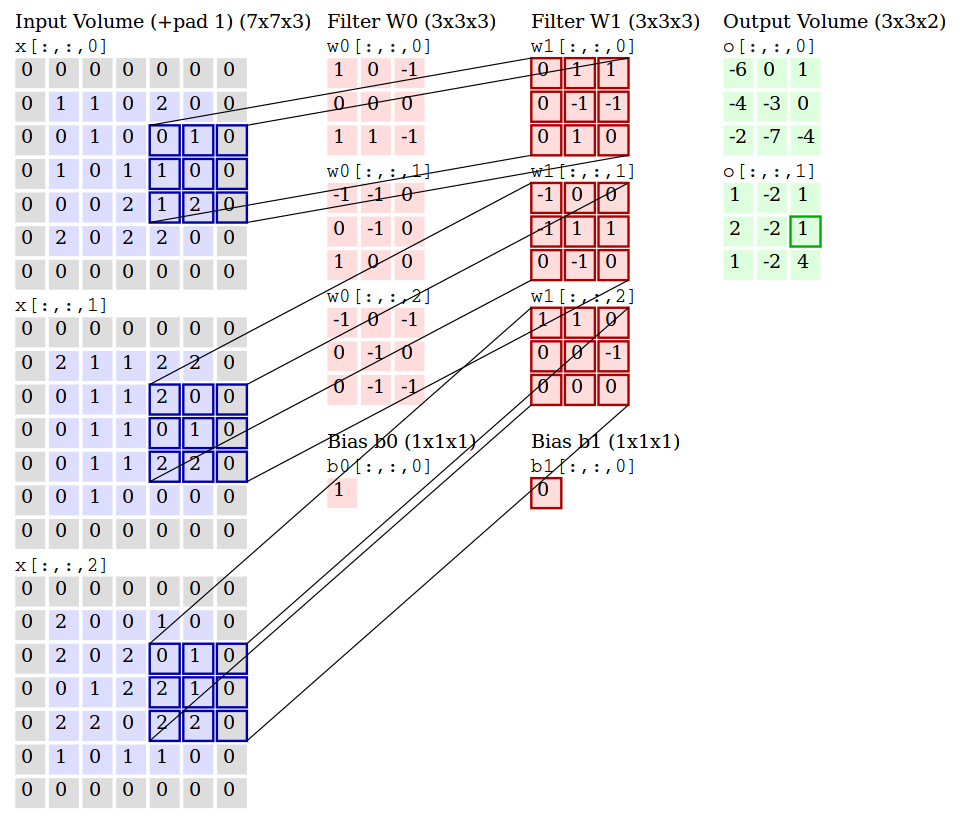
\includegraphics[scale=0.35]{images/filter_w1}
	\caption{Convolutional input with W1 filter}
	\label{figconvw1}
\end{figure}
\fi
\subsection{Pooling layer}
Pooling (POOL) layer  is another common layer in CNNs network. It is used to reduce the spatial size of the representation to reduce the quantity of the parameters and control overfitting. Hence, it performs a downsampling operation along the spatial dimensions (width, height). This operation will not affect to the depth dimension of the input. More generally, the POOL layer:
\begin{itemize}
	\item Accept a input of size \textbf{$W_1$ x $H_1$ x $D_1$}
	\item Requires two hyperparameters:
		\begin{itemize}
			\item Size of filter (spatial extent) \textbf{F} (commonly F = 4)
			\item The stride \textbf{S} (commonly S = 1)
		\end{itemize}
	\item The output with size of \textbf{$W_2$ x $H_2$ x $D_s$} where:
		\begin{itemize}
			\item \textbf{$W_2$ = $(W_1 - F)/S$ + $1$}
			\item \textbf{$H_2$ = $(H_1 - F)/S$ + $1$}
			\item \textbf{$D_2$ = $D_1$}
		\end{itemize}
	\item Note that it is not common to use zero padding for POOL layer since it computes a fixed function of the input.
\end{itemize}
The common function in POOL layer is \textbf{MAX} function and the size of filter is 2x2. The filter will slice over the input and using MAX operation over 4 number (in 2x2 region). Besides MAX function, the POOL layer can use the average function or L2-norm.
\begin{figure}[!h]
	\centering
	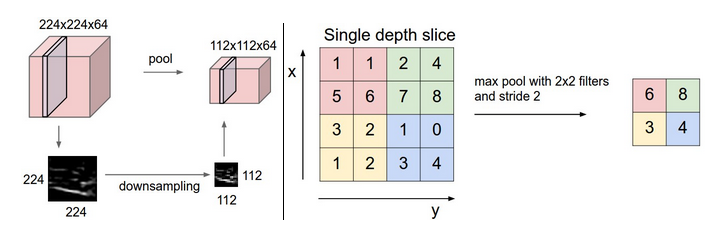
\includegraphics[scale=0.65]{images/pooling}
	\caption{A POOL layer with MAX function}
	\label{figconvw1}
\end{figure}

\subsection{Dropout layer}

\textbf{Dropout layer} \cite{} is a very specific layer in CNNs. As discussed in the previous section, \textbf{pooling layers} have really useful to control the overfitting problem, which has the good performance during the training process but does not perform when given the new data. However, the operation of max pooling is not enough strong to destroys the overfitting. So, dropout is another idea to help the network solves this problem. The idea of dropout is simplistic in nature. It dops out a random some activations in a layer by setting them to zero. By that, it makes the network to be redundant which makes sure that the network is not too ``fitted" to the training data and thus helps alleviate overfitting. Besides, dropout layer also improves the speed of the training process. A special thing is the neurons will be removed only during the training process. They are reinserted into the network with their original weights in the testing process.

\subsection{Full connected layer}
Full connected (FC) layer computes the class scores of the input. The neurons in FC layer have full connections to all activations in the previous layer. Their activations can be computed with a matrix multiplication followed by a bias offset.\\[0.2cm]
The difference between CONV and FC layer is that the neurons in the CONV layer are connected only to a local region in the input and the neurons in CONV layer are sharing parameters. However, the neurons in both layers still compute the dot products (it means the functional form is identical). Therefore, it turns out that it is possible to convert between FC and CONV layer.
\begin{itemize}
	\item For any CONV layer can be become a FC layer if we implement the same forward function. The weight matrix would be a large matrix that is mostly zero except for at certain blocks where the weights in many of the blocks are equal.
	\item Conversely, a FC layer can be converted to a CONV layer by setting the filter size to be exactly the size of the input and the output will be give identical result as the initial FC layer because only a single depth column fits across the input.
\end{itemize}
\section{Frameworks}
\subsection{Caffe}
Caffe is a deep learning framework in C++ that is developed by the Berkeley Vision and Learning Center (BVLC) and community contributors. Besides the supporting help user defined the network without hard-coding, easily to change the device machine (CPU or GPU), speedly, Caffe already has a large community user. These are reasons that Caffe is used in many research projects and many application in vision, speech and multimedia.

Caffe uses a definition of \textit{blobs} to store and to communicate data. It provides a uniform memory to hold data into the network. A network in Caffe is combined from the \textit{layers}. A layer take input from the bottom connection and through the output to top connection. For each layer of the network, the setting parameters are different depending on the type of layer. However, each layer type has the same of three critial computiations: \textbf{setup} initilize the layer and its connections; \textbf{forward} give the input from bottom connections, compute and send the output to the top connections; \textbf{backward} given the gradient from the top connections, compute the gradient and send to the bottom connections. Besides the network components, the information for training, optimizing the network are defined in \textbf{Solver} file.
\subsection{Theano}
Theano is a Python library that allows to define, optimize and evaluate mathematical expression involving multi-dimensional arrays efficiently \cite{}.
To realize this, the mathematical expressions which defined by the user are stored as a graph of variables and operations, that is pruned and optimized at compilation time. Like Caffe, Theano allows the users compile the program either on CPUs or GPUs.

\subsection{TensorFlow}
TensorFlow \cite{•} is an open source software library for numerical computation using data flow graphs. Each node in the graph represents for a mathematical operation, while the edge represents the communication between the data arrays(tensors). Tensorflow supports Python and C++, along to allow computing distribution among CPU, GPU and even horizontal scaling.
\subsection{Torch}
Torch \cite{•} is a scientific computing framework for machine learning. It is written by Lua language and an underlying C/CUDA implementation. At the heart of Torch is implemented the functions for neural network and optimization libraries. The user can build arbitrary graphs of neural networks and parallelize them over CPUs and GPUs in an efficient manner.
\subsection{PyTorch}
PyTorch \cite{} is a python package that provides two high-level features: 
\begin{itemize}
	\item Tensor computation with strong GPU acceleration
	\item Deep Neural Networks built on a tape-based autodiff system.
\end{itemize}
Most frameworks have a static view of the network. One has to build a neural network and reuse the same structure again. With PyTorch is different, the technique Reverse-mode auto differentiation allows to change the way of the network works aribitrary with zero lag or overhead. Additional, it integrate acceleration libraries such as Intel MKL and NVIDIA to maximize speed. At the core, the backend on CPU, GPU Tensor and Neural Network are written as independent libraries.
\subsection{Trends of Deep Learning libraries}
Fig. \ref{figtrendslibs} presents the trends of deep learing libraries in 2018. The color in the circle shows the age (in days) of the libraries from start date given on Github under Insights/Contributors (greener = younger, bluer = older). By all measures, TensorFlow is the leader. Keras, Caffe, Microsoft Cognitive Toolkit and PyTorch are in top five.

\begin{figure}[!h]
	\centering
	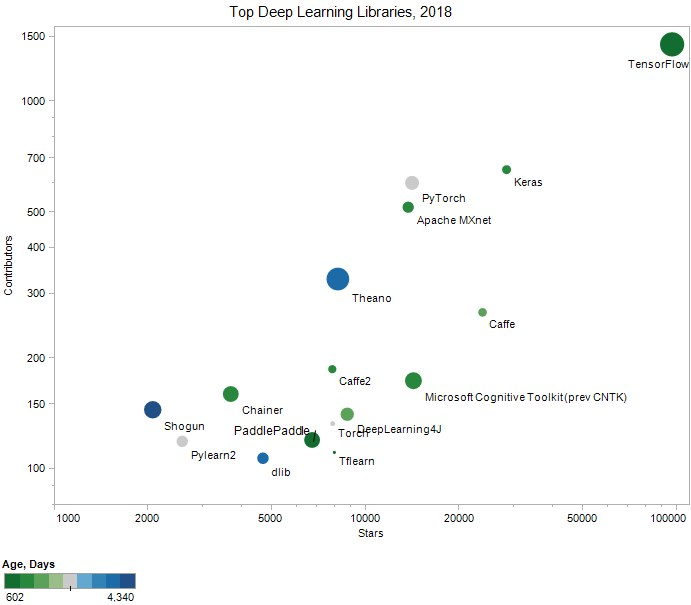
\includegraphics[scale=0.65]{images/trend_deep_learning_libs_2018}
	\caption{Top 16 open source deep learning libraries by Github stars and contributors}
	\label{figtrendslibs}
\end{figure}

\section{Case studies}
This section gives several architectures in the field of CNNs that we have.
\begin{itemize}
	\item \textbf{LeNet}: is developed by Yann Le Cun \cite{lecun1998gradient} in 1990's. It was used to read the zip code, digits.
	\item \textbf{AlexNet}: is developed by Alex Krizhevsky, Ilya Sutskever and Geoff Hinton \cite{krizhevsky2012imagenet}. This network had very similar architecture to LeNet, but was deeper, bigger and featured CONV layers stacked on top of each other.
	\item \textbf{ZF Net}: from Matthew Zeiler and Rob Fergus \cite{zeiler2014visualizing}. It was improved the AlexNet by tweaking the architecture hyperparameters (extending the size of the middle CONV layers and making the stride and the filter size on the first layer smaller).
	\item \textbf{GoogLeNet}: from Szegedy and al from Google \cite{szegedy2015going}. They develop an \textit{Inception Module} to reduce the number of parameters in the network. Additionally, they have used Average pooling instead of FC layers at the top of the CNN.
	\item \textbf{VGGNet}: is developed from Karen Simonyan and Andrew Zisserman\cite{simonyan2014very}. They show that the depth of the network is a critical component for good performance.
	\item \textbf{ResNet}: is developed by Kaiming He and al\cite{he2015deep}. The architecture of this network is missing FC layers at the end of network. It features skip connections and a heavy use of batch normalization\cite{ioffe2015batch}.
\end{itemize}

\iffalse
\section{Caffe framework}
Caffe is a deep learning framework that is developed by the Berkeley Vision and Learning Center (BVLC) and community contributors. Besides the supporting help user defined the network without hard-coding, easily to change the device machine (CPU or GPU), speedly, Caffe already has a large community user. These are reasons that Caffe is used in many research projects and many application in vision, speech and multimedia. This  section will describe the components and the architecture of Caffe. We also using Caffe to create a small network for classification.
\subsection{Definitions}
Deep network is a model that represented as a collection of inter-connected layers. Keep this definition, Caffe defines a network layer by layer in its model. The data through in the network called \texttt{blobs}. Blobs is the standard array and unified memory interface for the framework. The layer is the foundation of the model and computation. The net is defined as the collection of connection between the layers. The structure of blob will describe the way that information is stored and communicated in the layers and networks.
\subsubsection{Blobs}
Caffe stores and communicates data using blobs. Blobs provide a uniform memory to hold data. The blob dimensions for batches of an image are number \textbf{N} x channel \textbf{K} x height \textbf{H} x width \textbf{W}. Where:
\begin{itemize}
	\item Number N: is the batch size of the data (the number of data through the network in the same time).
	\item Channel K: is the feature dimension of image (i.e for RGB image K = 3)
	\item Width W and height H: are width and height of the image data.
\end{itemize}
In Caffe, the dimension of blob is dependent on the type and configuration of the layer.
\subsubsection{Layers}
The layer is the principle of the model and the fundamental unit of computation. Caffe has provided a lot of layer's type as convolution, pool, inner products,etc. But most of types have the same model as figure \ref{figcaffelayer}. A layer take input from the bottom connections and through the output to top connections. Each layer type defines three critical computations:
\begin{itemize}
	\item \textbf{Setup}: initialize the layer and its connections.
	\item \textbf{Forward}:  given the input from bottom connections, compute and send the output to the top connections.
	\item \textbf{Backward}: given the gradient from the top connection, compute the gradient to the input and send to the bottom connections.
\end{itemize}
\begin{multicols}{2}
[An example about declaring a layer in Caffe and its model:\\]
\texttt{
layer $\lbrace \\
  \text{\tab\tab} name: ``conv1"\\
  \text{\tab\tab}type: ``Convolution"\\
  \text{\tab\tab}bottom: ``data"\\
  \text{\tab\tab}top: ``conv1"\\
  \text{\tab\tab}param \lbrace\\
  \text{\tab\tab\tab}lr\_mult: 1\\
  \text{\tab\tab}\rbrace\\
  \text{\tab\tab}param \lbrace\\
  \text{\tab\tab\tab}lr_mult: 2\\
  \text{\tab\tab}\rbrace\\
  \text{\tab\tab}convolution\_param \lbrace\\
  \text{\tab\tab\tab}num\_output: 20\\
  \text{\tab\tab\tab}kernel\_size: 5\\
  \text{\tab\tab\tab}stride: 1\\
  \text{\tab\tab\tab}weight\_filler \lbrace\\
  \text{\tab\tab\tab\tab}type: "xavier"\\
  \text{\tab\tab\tab}\rbrace\\
  \text{\tab\tab\tab}bias\_filler \lbrace\\
  \text{\tab\tab\tab\tab}type: "constant"\\
  \text{\tab\tab\tab}\rbrace\\
  \text{\tab\tab}\rbrace\\
\text{\tab}\rbrace$
}
\columnbreak
\begin{wrapfigure}{l}{0.9\linewidth}
	\centering
	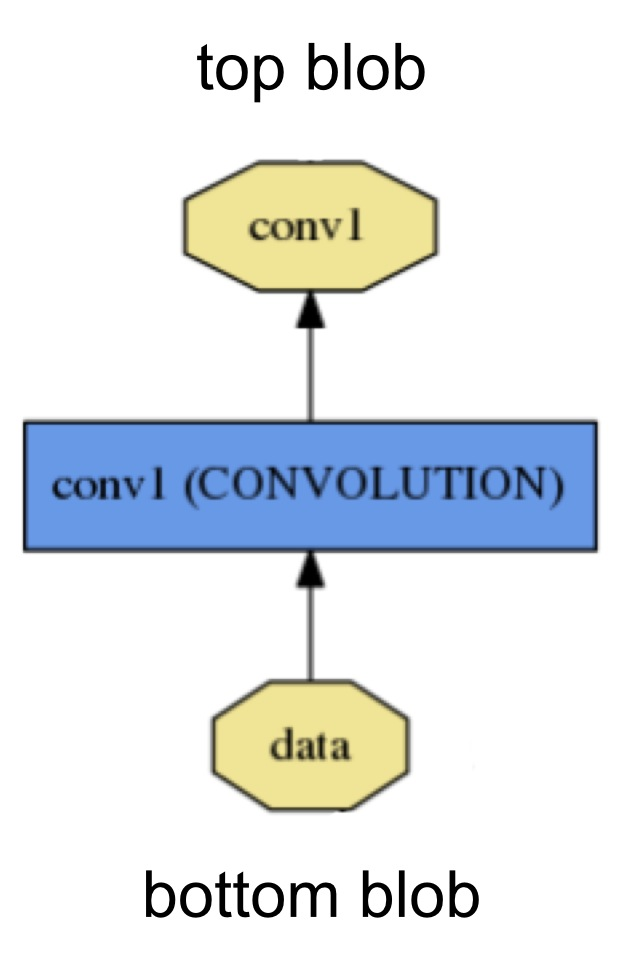
\includegraphics[scale=0.45]{images/caffelayer}
	\caption{Model of a layer in Caffe framework}
	\label{figcaffelayer}
\end{wrapfigure}
\end{multicols}
\subsubsection{Nets}
The net is a set of layers connected in a computation directed acyclic graph. A net begins with a data layer that loads the data from the disk and ends with a loss layer that computes the objective of the network (such as classification, recognition,...). As simple, a net is defined as figure \ref{figcaffenet}.
\begin{figure}[!h]
	\centering
	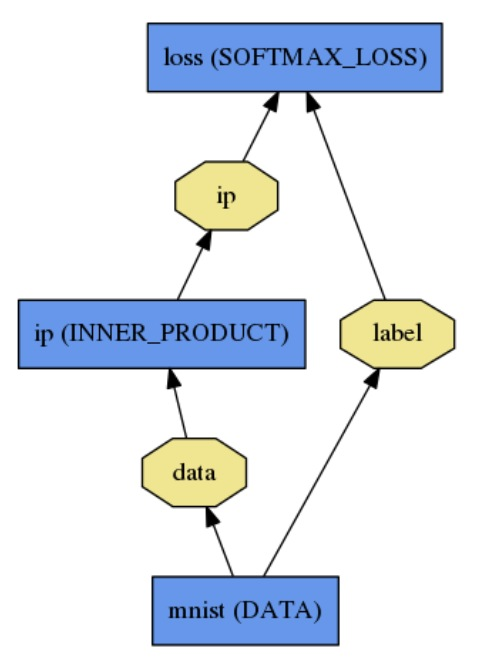
\includegraphics[scale=0.5]{images/caffenet}
	\caption{Model of a net in Caffe framework}
	\label{figcaffenet}
\end{figure}
\subsubsection{Forward pass}
Forward pass computes the output given the input by the functions. Each function stays at each layer of the model. The forward pass through from bottom to the top via each layer of model. The image \ref{figforward} shows a forward example. The input data \textit{x} through the \textbf{Inner Product} layer and \textbf{Softmax} layer to give the last result. Normally, the output of forward pass includes the result of score function and the error (loss) of the model.
\begin{figure}[!h]
	\centering
	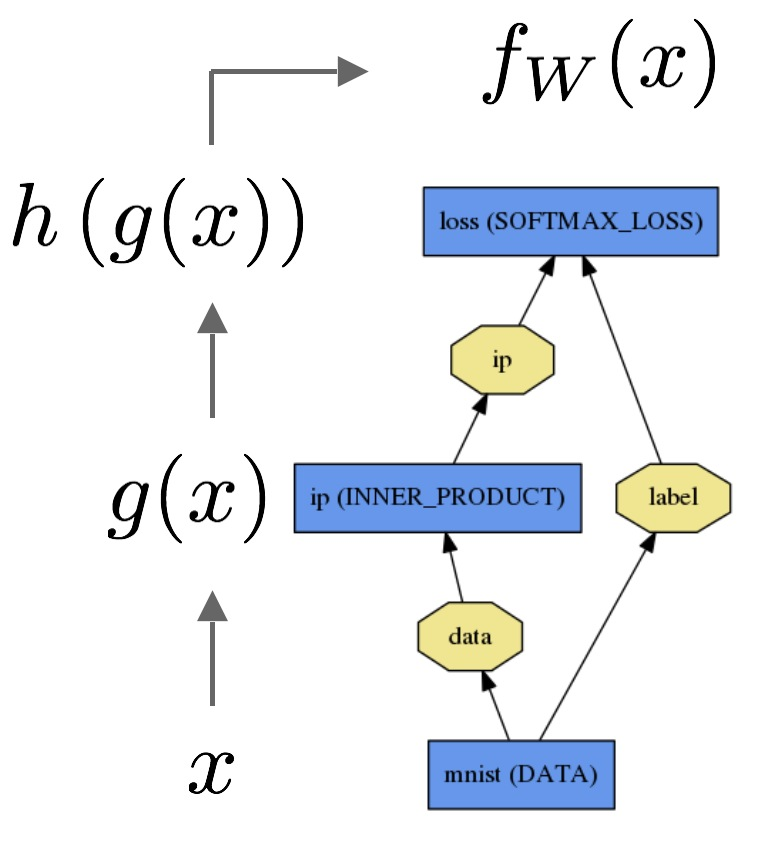
\includegraphics[scale=0.45]{images/forward}
	\caption{Forward pass in a Caffe model}
	\label{figforward}
\end{figure}
\subsubsection{Backward pass}
Backward pass receives the loss as the input, it computes the gradient for learning of the model. The gradient of the model is computed by inverse-compose gradient of each layer in the model. Backward pass through from top to bottom. The gradient respect of the model is computed layer by layer via the chain rule through the parameters of each layer (figure \ref{figbackward}).
\begin{figure}[!h]
	\centering
	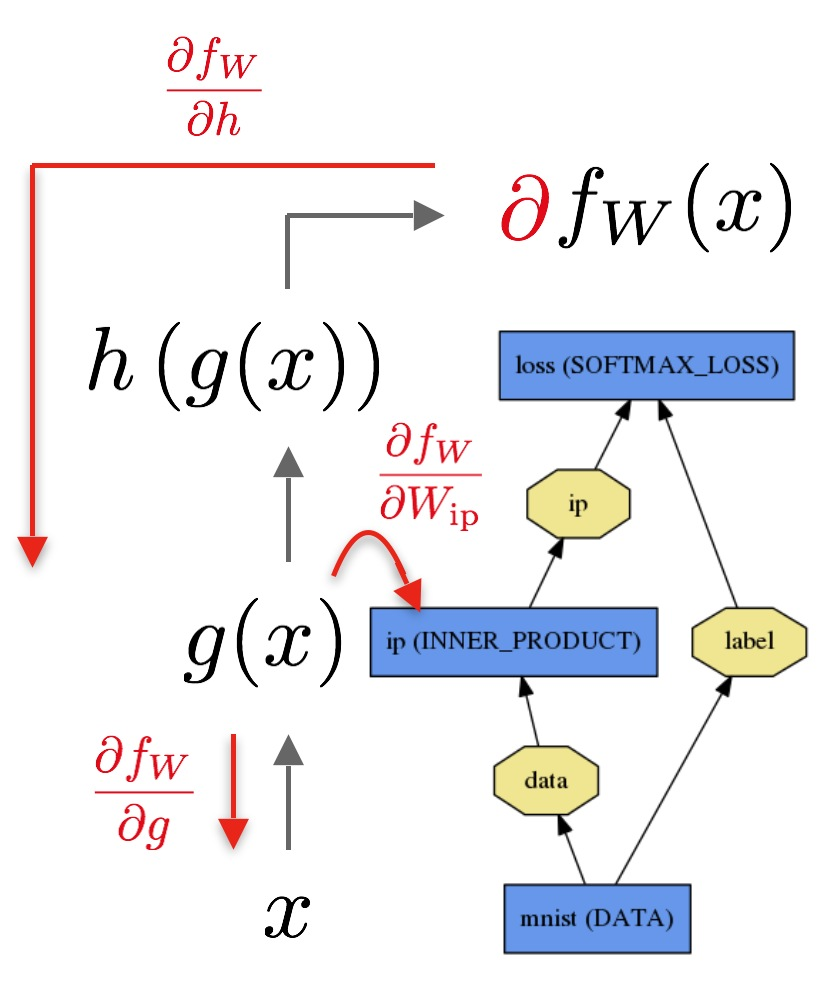
\includegraphics[scale=0.45]{images/backward}
	\caption{Backward pass in a Caffe model}
	\label{figbackward}
\end{figure}
\subsubsection{Solver}
In Caffe, Solver is designed for optimizing the model by coordinating the network's forward inference and backward gradients to form parameter update that attempt to improve the loss. The steps in optimizing process are followed:
\begin{itemize}
	\item Firstly, calling the forward pass to obtain the output and loss,
	\item Secondly, calling the backward pass to generate the gradient of model,
	\item Finally, Incorporating the gradient into the weight update that attempts to minimize the loss.
\end{itemize}
The Caffe solvers include:
\begin{itemize}
	\item Stochastic Gradient Descent
	\item AdaDelta
	\item Adaptive Gradient
	\item Adam
	\item Nesterov's Accelerated Gradient
	\item RMSprop
\end{itemize}
\section{Layers Catalogue}
The layers in Caffe framework are organized similarly to CSS language. They are defined following the structure with the specific attributes. The model architecture of a network using Caffe is defined in a protocol buffer definition file (prototxt). In general, the structure of a layer in Caffe looks like:\\
\texttt{
layer $\lbrace \text{\tab \# \textbf{layer} is keyword}\\
  \text{\tab\tab} name: ``\text{\textbf{name}}" \text{\tab \# Name of layer}\\
  \text{\tab\tab}type: ``layer\_type" \text{\tab \# Type of layer}\\
  \text{\tab\tab}bottom: ``bottom\_blob" \text{\tab \# Input (bottom) of layer}\\
  \text{\tab\tab}top: ``top\_blob" \text{\tab \# Output (top) of layer}\\
  \text{\tab\tab \# And the parameters of layer(required, recommended or optional parameters)}\\
\text{\tab}\rbrace$
}\\[0.2cm]
Depending to specific layer, Caffe has provided difference parameters. This section will discuss a few of the important layers.
\subsubsection{Convolution layer}
The convolution layer means applying a mathematical function to a range of image. The aim of this function is convolutional the image with a new depth. The parameters of this layer are as followed:
\begin{itemize}
	\item Layer type: \texttt{Convolution}
	\item Required parameters:
		\begin{itemize}
			\item \texttt{num\_output(n)}: the number of filters
			\item \texttt{kernel\_size}: specifies width and height of each filter
		\end{itemize}
	\item Recommended parameters: \texttt{weight\_filler} has two sub-parameters: \texttt{type} and \texttt{value}.This is an initialization for filter)
	\item Optional parameters:
		\begin{itemize}
			\item \texttt{stride}: specifies the moving-step when applying the filters to the input.
			\item \texttt{bias\_term}: specifies the addition biases to the outputs.
			\item \texttt{pad}: specifies the addition pixels to each side of the input.
			\item \texttt{group(g)}: Indicating the connectivity of each filter to a subset of the input.
		\end{itemize}
\end{itemize}
An example of convolution layer (fig.\ref{figstconv}):
\begin{figure}[!h]
	\centering
	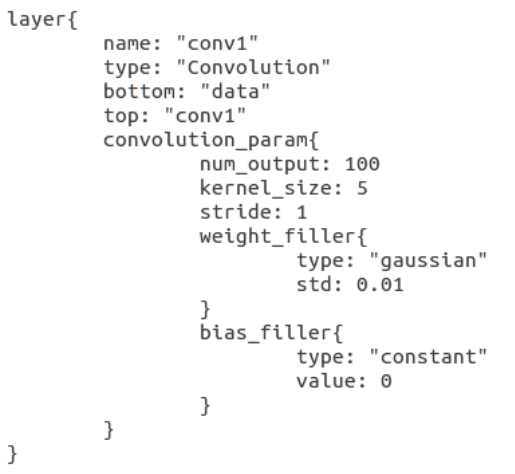
\includegraphics[scale=0.4]{images/stconv}
	\caption{A convolution layer in Caffe}
	\label{figstconv}
\end{figure}
\subsubsection{Pooling layer}
The pooling layer works similar to a convolution layer but the functions at pooling layer are different (maximum function (MAX) or average function (AVE)). The parameters of pooling layer are followed:
\begin{itemize}
	\item Layer type: \texttt{Pooling}
	\item Required parameter: \texttt{kernel\_size} specifies width and height of each filter
	\item Optional parameters:
		\begin{itemize}
			\item \texttt{pool}: the pooling method, such as: \textbf{MAX, AVE, STOCHASTIC}.
			\item \texttt{pad}: specifies the pixels to add to each side of the input.
			\item \texttt{stride}: moving-step when applying the filters to the input
		\end{itemize}
\end{itemize}
An example of pooling layer (fig. \ref{figstpool}):
\begin{figure}[!h]
	\centering
	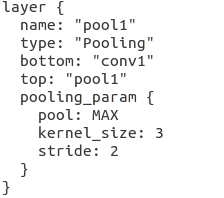
\includegraphics[scale=0.7]{images/stpool}
	\caption{A pooling layer in Caffe}
	\label{figstpool}
\end{figure}
\subsubsection{Loss layers}
Loss of learning is indicated by comparing an output to a target and assigning cost to minimize. The loss computed includes the loss in forward pass and the gradient in backward pass. The loss functions in Caffe are described as followed:
\begin{itemize}
	\item \textbf{Softmax} (layer type: \texttt{SoftmaxWithLoss})
	\item \textbf{Euclidean} (layer type: \texttt{EuclideanLoss})
	\item \textbf{Hinge/Margin} (layer type: \texttt{HingeLoss})
	\item \textbf{Sigmoid Cross-Entropy} (layer type: \texttt{SigmoidCrossEntropyLoss})
	\item \textbf{Infogain} (layer type: \texttt{Infogain})
\end{itemize}
Example about a loss layer using \textbf{Softmax} (fig. \ref{figstloss}):
\begin{figure}[!h]
	\centering
	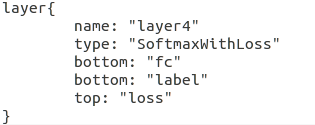
\includegraphics[scale=0.7]{images/stloss}
	\caption{A loss layer in Caffe}
	\label{figstloss}
\end{figure}
\subsubsection{Activation layers}
Activation layers are taking one bottom blob and producing one top blob of the same size with an activation function. The activation function in Caffe includes:
\begin{itemize}
	\item \textbf{ReLU} (layer type:\texttt{ReLU})
	\item \textbf{Sigmoid} (layer type:\texttt{Sigmoid})
	\item \textbf{TanH} (layer type:\texttt{TanH})
	\item \textbf{Absolute} (layer type:\texttt{AbsVal})
	\item \textbf{Power} (layer type:\texttt{Power})
	\item \textbf{BNLL} (layer type:\texttt{BNLL})
\end{itemize}
An activation layer with ReLU (fig. \ref{figstrelu}):
\begin{figure}[!h]
	\centering
	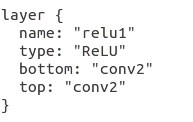
\includegraphics[scale=0.7]{images/strelu}
	\caption{A ReLU layer in Caffe}
	\label{figstrelu}
\end{figure}
\subsubsection{Inner Product layer}
This is a fully connected layer of Caffe. The parameters of this layer are followed:
\begin{itemize}
	\item Layer type: \texttt{InnerProduct}
	\item Required parameter: \texttt{num\_output(c\_o)} the number of filters
	\item Recommended parameter: \texttt{weight\_filler} initialize of filters.
	\item Optional parameters:
		\begin{itemize}
			\item \texttt{bias\_filler}: initialize of bias filters
			\item \texttt{bias\_term}: specifies whether to learn and apply a set of additive biases to the filter outputs.
		\end{itemize}
\end{itemize}
An example of inner product layer (fig. \ref{figstinner}):
\begin{figure}[!h]
	\centering
	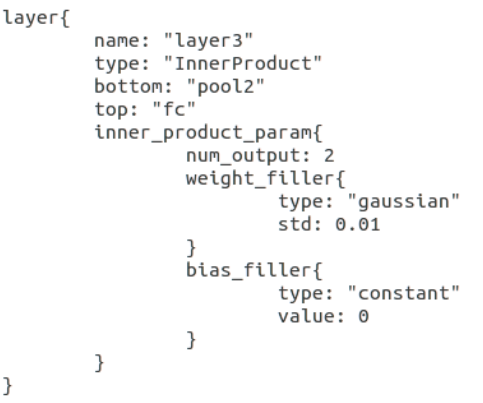
\includegraphics[scale=0.5]{images/stinner}
	\caption{An Inner Product layer in Caffe}
	\label{figstinner}
\end{figure}
\subsubsection{Data layer}
Data enters Caffe through data layers. They lie at the bottom of nets. Caffe strongly supports many kinds of data, directly from memory or from files on disk in HDF5 or common image formats. The types of data are include:
\begin{itemize}
	\item \textbf{Database}: layer type \texttt{Data}
		\begin{itemize}
			\item Required parameters:
				\begin{itemize}
					\item \texttt{source}: the name of the directory containing the database
					\item \texttt{batch\_size}: the number of inputs to process at one time
				\end{itemize}
			\item Optional parameters:
				\begin{itemize}
					\item \texttt{rand\_skip}: skip up to this number of inputs at the beginning
					\item \texttt{backend}: choose whether to use a \textbf{LEVELDB} or \textbf{LMDB}
				\end{itemize}
		\end{itemize}
	\item \textbf{In-Memory}: layer type \texttt{MemoryData}. Required parameters: \texttt{batch\_size, channels, height, width} - specify the size of input chunks to read from memory
	\item \textbf{HDF5 Input}: layer type \texttt{HDF5Data}. Required parameters are followed:
		\begin{itemize}
			\item \texttt{source}: the name of the file to read from
			\item \texttt{batch\_size}: number of images to batch together
		\end{itemize}
	\item \textbf{HDF5 Output}: layer type \texttt{HDF5Output}. Required parameter are \textbf{file\_name} which name of file to write the output.
	\item \textbf{Images}: layer type \texttt{ImageData}.
		\begin{itemize}
			\item Required parameters:
				\begin{itemize}
					\item \texttt{source}: name of a text file. Each line gives an image filename and label
					\item \texttt{batch\_size}: number of images to batch together
				\end{itemize}
			\item Optional parameters:
				\begin{itemize}
					\item \textbf{rand\_skip}: skip up to this number of inputs at the beginning
					\item \texttt{shuffle}
					\item \texttt{new\_height, new\_width}: resize all images to this size
				\end{itemize}
		\end{itemize}
\end{itemize}
An example of data layer:
\begin{figure}[!h]
	\centering
	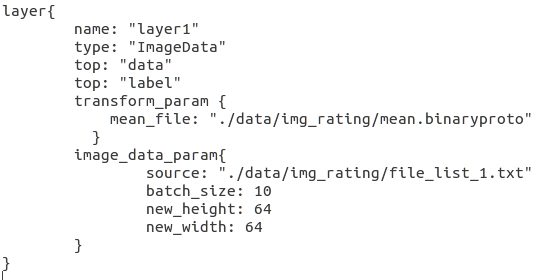
\includegraphics[scale=0.65]{images/stdata}
	\caption{A data layer in Caffe}
	\label{figstdata}
\end{figure}
\fi

\section{A small deep network with Caffe}
Caffe uses prototxt format for specification of neural networks. Each layer is defined separately with the inputs, the outputs called blobs. The layers are stacked vertical with the input of layer at the bottom and the output of layer at the top. Besides, each layer expects a number of input and output blobs. The figure xx show an sample deep neural netwoks. The network begin the input layer that takes the data input, an output of network that computes the final prediction, a loss layer which can be intergrated with the final output layer. We will discuss how to create this network by Caffe.\\[0.2cm]

The first layer in the network is the input layer. In this network, the ImageData has been used. It takes an input text file which contains multiple lines of input. Each line contains the path to each image and its label, separated as a space. Besides ImageData, we can use other input layers which are supported by Caffe such as HDF5, Data,...\\[0.2cm]

The second layer is a convolutional layer. In this sample, we choose \textit{kernel\_size} as nine with a \textit{stride} of three and the number of outputs will be set to 100. This layer take the output of the first layer as the input, then its output will be used at next layer. The parameters depend on how deep the convolutional layer is placed in the network and what level of detail of features is begin targeted.\\[0.2cm]

The third layer is a fully connected layer which generates a prediction on the labels possible. The number of output is equal to the number of labels.\\[0.2cm]

The fourth and fifth layer is the Sofmax and output layer. The layers use softmax distribution on the output of fully connected layer to compute the probabilities of the image belonging to each label. Besides, the layer also compute the loss for backpropagation for training.\\[0.2cm]

Now, we have finished design network. Now, we will Caffe to create a real network. The stages to create network as follows:
\begin{enumerate}
	\item Preparing the dataset: collect the images and place them in a directory. Then, create a text file with all the image names and its label.
	\item Creating the network: The layers are stacked as description above in a file and saving in a \textbf{prototxt} format.
	\item Create a solver file to describe the step learning procedure.
	\item Star the training procedure with command \\
	\texttt{build/tools/caffe train --solver=./path/to/solver.protoxt --gpu=0}
\end{enumerate}
After finishing the training procedure, a file with format caffemodel will be generated. We use this file as model of the network in specifies program.